\documentclass{article}
\usepackage{graphicx}
\usepackage{amsmath}
\usepackage{enumitem}
\usepackage{float}
\usepackage{listings}
\usepackage{xcolor}
\usepackage{caption}
\usepackage[a4paper, margin=1in]{geometry}

% Custom information
\newcommand{\className}{Course: Automatic Control Systems – ASEN 5114-001 – Spring 2025}
\newcommand{\professorName}{Professor: Dale Lawrence}
\newcommand{\taName}{Teaching Assistant: Anantha Dhruva}
\title{Project 1 \\ \className \\ \professorName \\ \taName}
\author{Steve Gillet}
\date{\today}

\lstdefinestyle{matlabstyle}{
    language=Matlab,              % Specify the language
    basicstyle=\ttfamily\footnotesize\color{black}, % Code font
    keywordstyle=\color{blue}\bfseries, % Keywords in blue
    stringstyle=\color{orange},    % Strings in orange
    commentstyle=\color{magenta}, % Comments in magenta
    numbers=left,                 % Line numbers on the left
    numberstyle=\tiny\color{black},% Line number style
    stepnumber=1,                 % Line number increment
    breaklines=true,              % Line breaking
    frame=single,                 % Border around code
    backgroundcolor=\color{white},
    tabsize=4,                    % Tab size
    showstringspaces=false,       % Don't show spaces in strings
}

\renewcommand{\thesection}{\arabic{section})}
\renewcommand{\thesubsection}{\arabic{section}.\alph{subsection})}

\begin{document}

\maketitle

\textit{The purpose of this project is to apply frequency domain modeling and design methods to control attitude of a spacecraft mockup. A combination of analytic and empirical modeling will be used to obtain a transfer function representation of the spacecraft dynamics. A controller will then be designed using frequency response methods, then implemented in a simulation of the hardware mockup. Predicted responses will be compared to simulated responses. Colocated versus non-colocated control issues will be explored.
The project can be carried out individually, or in small teams. Team projects (up to 3 team members) will submit a single report, and all members of a team project will receive the same grade. The report should include an introduction, separate sections for each of the following parts, and a conclusion pointing out interesting aspects or difficulties. All team members should contribute approximately equally to the conduct of the project and the write-up. Provide a statement of individual contributions in the report. The report is due Monday, April 7 at 11:59 PM.}

\section{}

\textit{[20 pts] Develop an analytic transfer function model to match the empirical frequency response obtained from the spacecraft mockup hardware (data posted on Canvas), for frequencies up through the first resonance/anti-resonance.}

The data came in the form of magnitudes (in (rad/s)/V) and phases (in rads) for a set of frequencies (Hz).
I started by converting the system to output radians by inserting an integrator block as seen in the diagram below, then converting the readings using the resulting transfer function.

\begin{figure}[H]
    \centering
    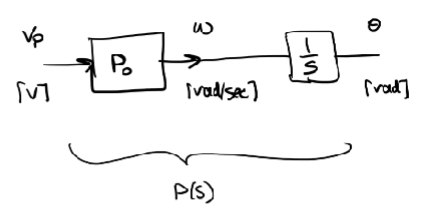
\includegraphics[width=0.8\textwidth]{dataIntegrationDiagram.png}
    \caption{Block diagram of the system.}
    \label{fig:dataIntegrationDiagram}
\end{figure}

The transfer function \(P(s)\) is given by:
\[
P(s) = P_0(s) \cdot \frac{1}{s}
\]
given \(|P_0(j\omega)|\), \(\angle P_0(j\omega)\) in radians.

For \(P_0(j\omega)\):
\[
P(j\omega) = P_0(j\omega) \cdot \frac{1}{j\omega}
\]

The magnitude in decibels is:
\[
|P(j\omega)|_{\text{dB}} = 20 \log_{10} |P_0(j\omega)| - 20 \log_{10} \omega
\]

The phase is:
\[
\angle P(j\omega) = \angle P_0(j\omega) - \angle \frac{1}{j\omega} = \angle P_0(j\omega) - 90^\circ
\]

I converted and plotted the resulting magnitudes (in dB) and phases (degrees) for the frequencies (in rad/s) to get the Bode plot of the system using the following MATLAB code:

\begin{lstlisting}[style=matlabstyle]
dataTable = readtable('data.xlsx');
data = table2array(dataTable);

n = size(data,1);
pResponse = zeros(n,3);

for i = 1:n
    pResponse(i,1) = 20*log10(data(i,2)) - 20*log10(data(i,1));
    pResponse(i,2) = data(i,3)*180/pi - 90;
    pResponse(i,3) = data(i,1)*2*pi;
end
\end{lstlisting}

\begin{figure}[H]
    \centering
    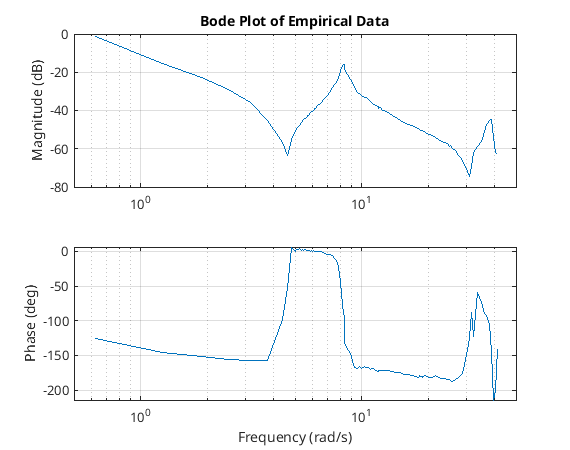
\includegraphics[width=0.8\textwidth]{empiricalBodePlot.png}
    \label{fig:empiricalBodePlot}
\end{figure}

In order to match an analytic model to the empirical data, I started with the most notable features, the resonance and antiresonance.
I knew that in order to get that resonance behavior you needed a term like a second-order polynomial of the form \((s^2 + 2\zeta\omega_n s + \omega_n^2)\), one in the numerator for the antiresonance and one in the denominator for the resonance.
I knew that the frequency of the peak of a resonance corresponds to the square of the natural frequency ($\omega_n$) so I set those to match the data and then tuned the damping ratio (\(\zeta\)) to get the right peak values and shape of the curve.

Then I realized that I needed to add a gain compensator K to move the transfer function up and down and I needed a couple of extra poles to get the -40 dB/decade slope in the magnitude and to bring the phase down to -180 degrees.
The resulting magnitude plot looked pretty close but in the empirical data there was this phase lagging behavior that you couldn't see at all in the analytical model:

\begin{figure}[H]
    \centering
    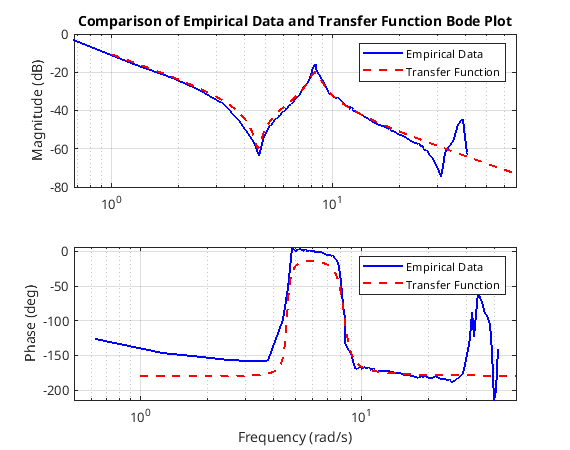
\includegraphics[width=0.8\textwidth]{flatPhaseBode.png}
    \label{fig:flatPhaseBode}
\end{figure}

So I decided to change one of the poles to have that $\frac{1}{s+b}$ lagging behavior and I set b to 0.65 so that it would kick in soon enough to effect low frequency phase while still achieving the -40 dB/decade slope in the magnitude.
So put together all of those terms and the resulting transfer function looks like: $\frac{K*(s^2 + 2\zeta\omega_n s + \omega_n^2)}{(s^2 + 2\zeta\omega_n s + \omega_n^2)(s)(s+b)}$.
I tweaked the parameters as described above to get a good fit so the transfer function ended up looking like: $\frac{K*(s^2 + 2*0.05*4.60118 s + 4.60118^2)}{(s^2 + 2*0.1*8.34686 s + 8.34686^2)(s)(s+0.65)}$.
And I implemented that in Matlab as such:

\begin{lstlisting}[style=matlabstyle]
K = 1;
zetaZ = 0.05;
zetaP = 0.1;
omegaZ = 4.60118;
omegaP = 8.34686;

num = K*[1 zetaZ*omegaZ omegaZ^2];
den = [1 zetaP*omegaP omegaP^2 0];
pole = [1 0.65];
den = conv(den, pole);
estTF = tf(num,den);
\end{lstlisting}

The final result looks like this:

\begin{figure}[H]
    \centering
    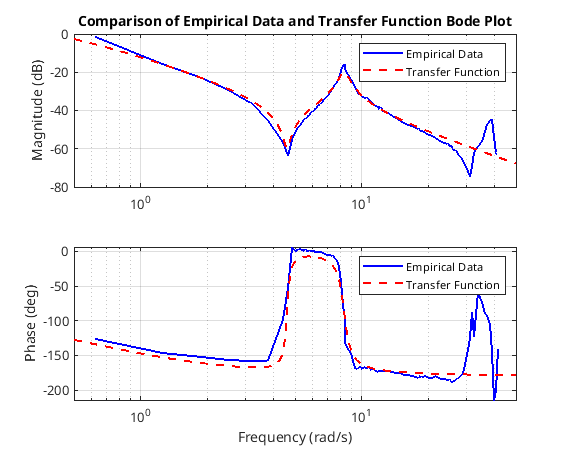
\includegraphics[width=0.8\textwidth]{analyticTFbode.png}
    \label{fig:analyticTFbode}
\end{figure}

Which looks pretty close and all of the important frequencies like the gain crossover frequency and resonance peak frequencies match up closely so that I am satisfied enough that the behavior will be the same.

\section{}

\textit{[20 pts] Examine the two loop transfer functions (analytic and empirical) via Bode plots and Nyquist plots using a proportional controller \(C(s) = K\). Would the control system be stable for some values of \(K\)? For all values of \(K\)?}

So you can see the Bode plots above, I also plotted the Nyquist plots using the 'nyquist' function in matlab for the analytical and converted the frequency response to complex form for the empirical plot using the following conversion: 
\[C(j\omega)G(j\omega) = K |G(j\omega)| \cos(\phi(\omega)) + j K |G(j\omega)| \sin(\phi(\omega))\]
The Matlab code for that conversion/plotting looks like this:

\begin{lstlisting}[style=matlabstyle]
realPart = K*10.^(pResponse(:,1) / 20) .* cosd(pResponse(:,2));
imagPart = K*10.^(pResponse(:,1) / 20) .* sind(pResponse(:,2));

figure;
plot(realPart, imagPart, 'b', 'LineWidth', 1.5);
hold on;
plot(realPart, -imagPart, 'b--', 'LineWidth', 1.5);
\end{lstlisting}

The results look like this:

\begin{figure}[H]
    \centering
    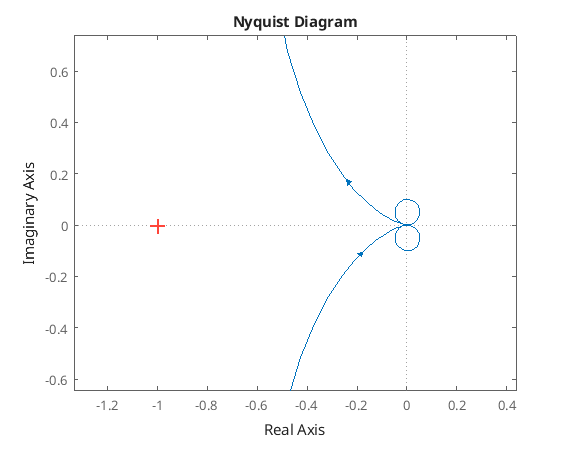
\includegraphics[width=0.8\textwidth]{nyquistAnalytic.png}
    \label{fig:nyquistAnalytic}
\end{figure}

\begin{figure}[H]
    \centering
    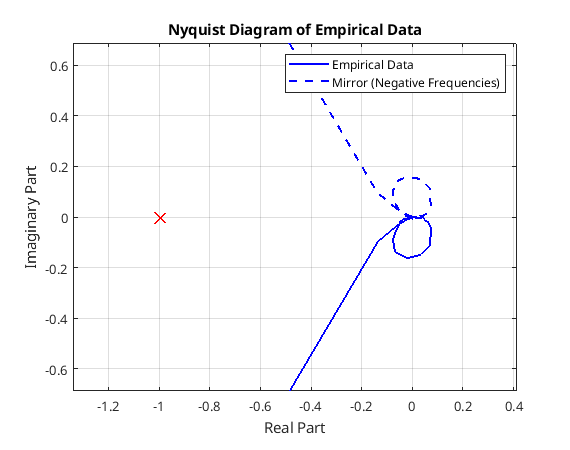
\includegraphics[width=0.8\textwidth]{nyquistEmpirical.png}
    \label{fig:nyquistEmpirical}
\end{figure}

Which look pretty similar which I was happy about.
I also drew the Nyquist plot and diagram of the analytic transfer function by hand so that we could see what is going on around infinite to get an idea of the encirclements.

\begin{figure}[H]
    \centering
    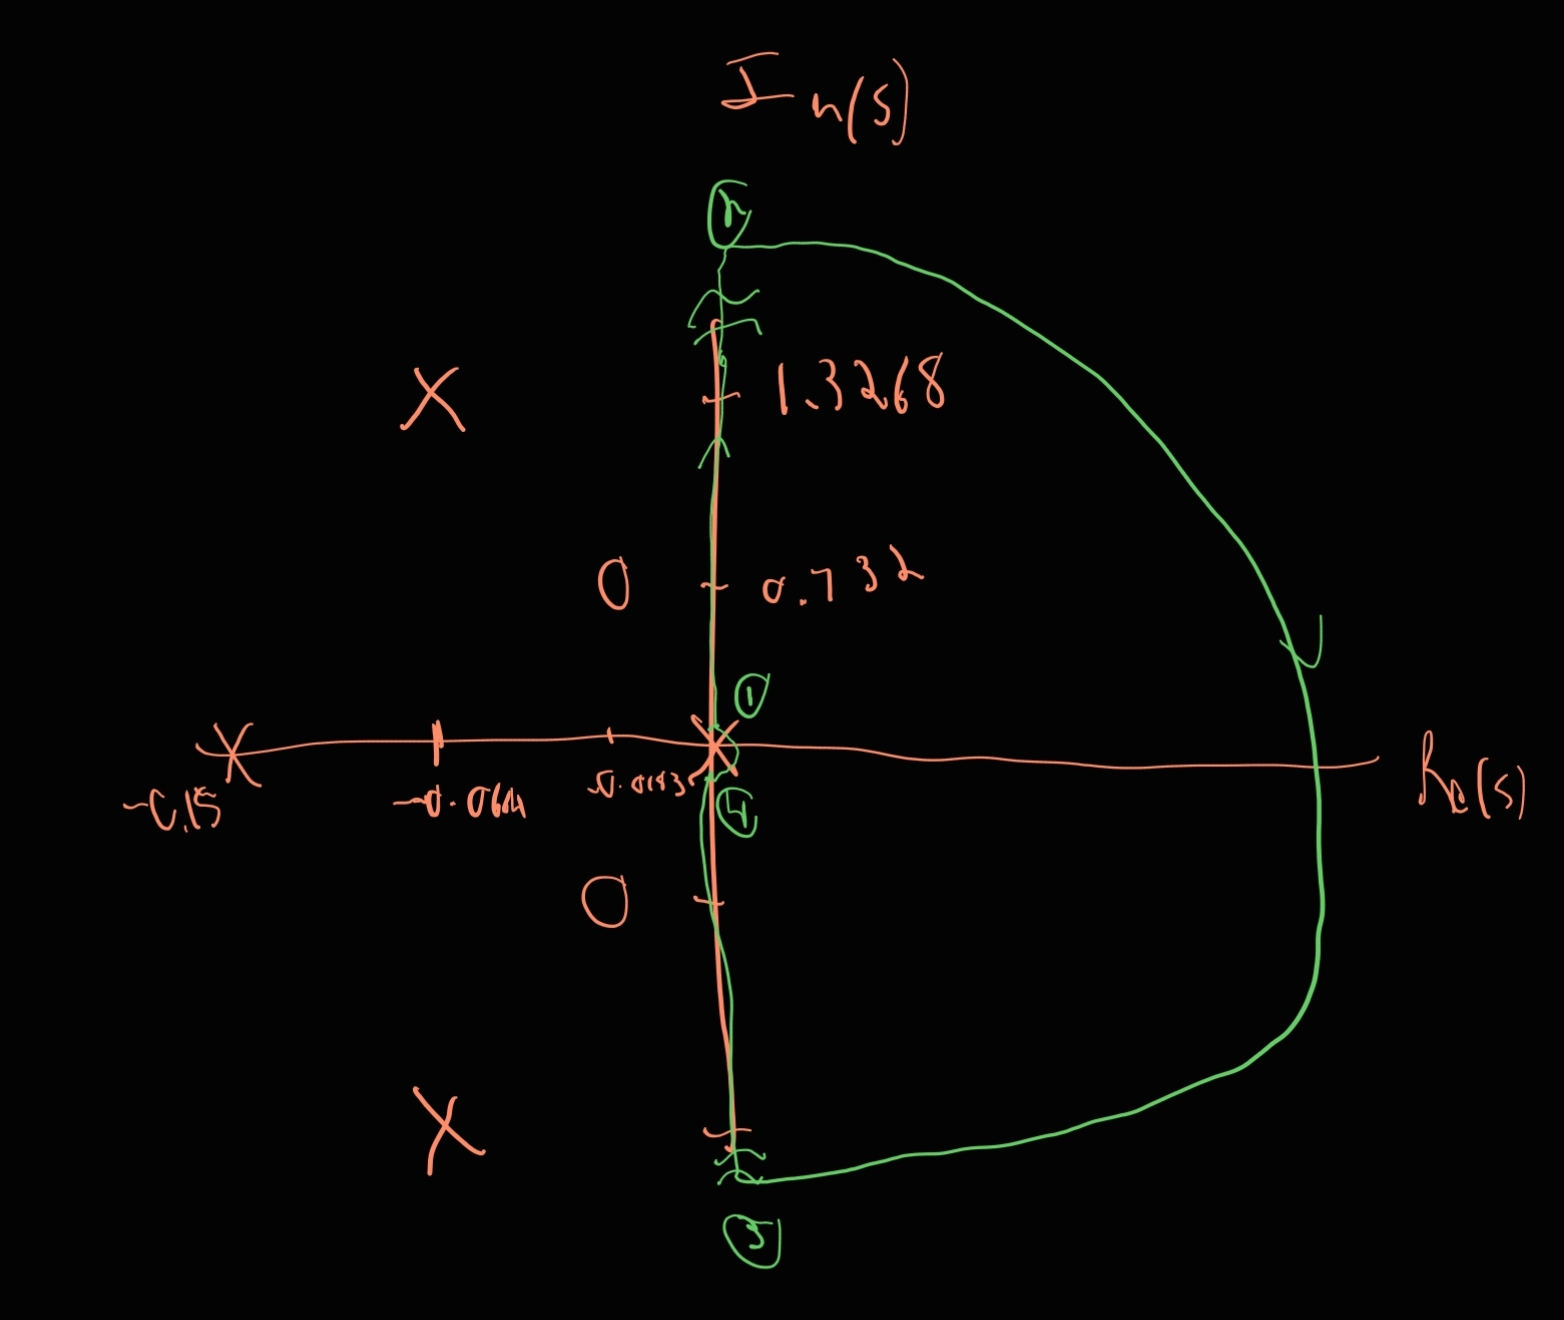
\includegraphics[width=0.8\textwidth]{nyquistPlot.jpg}
    \label{fig:nyquistPlot}
    \caption{Nyquist Plot of Analytic TF}
\end{figure}

\begin{figure}[H]
    \centering
    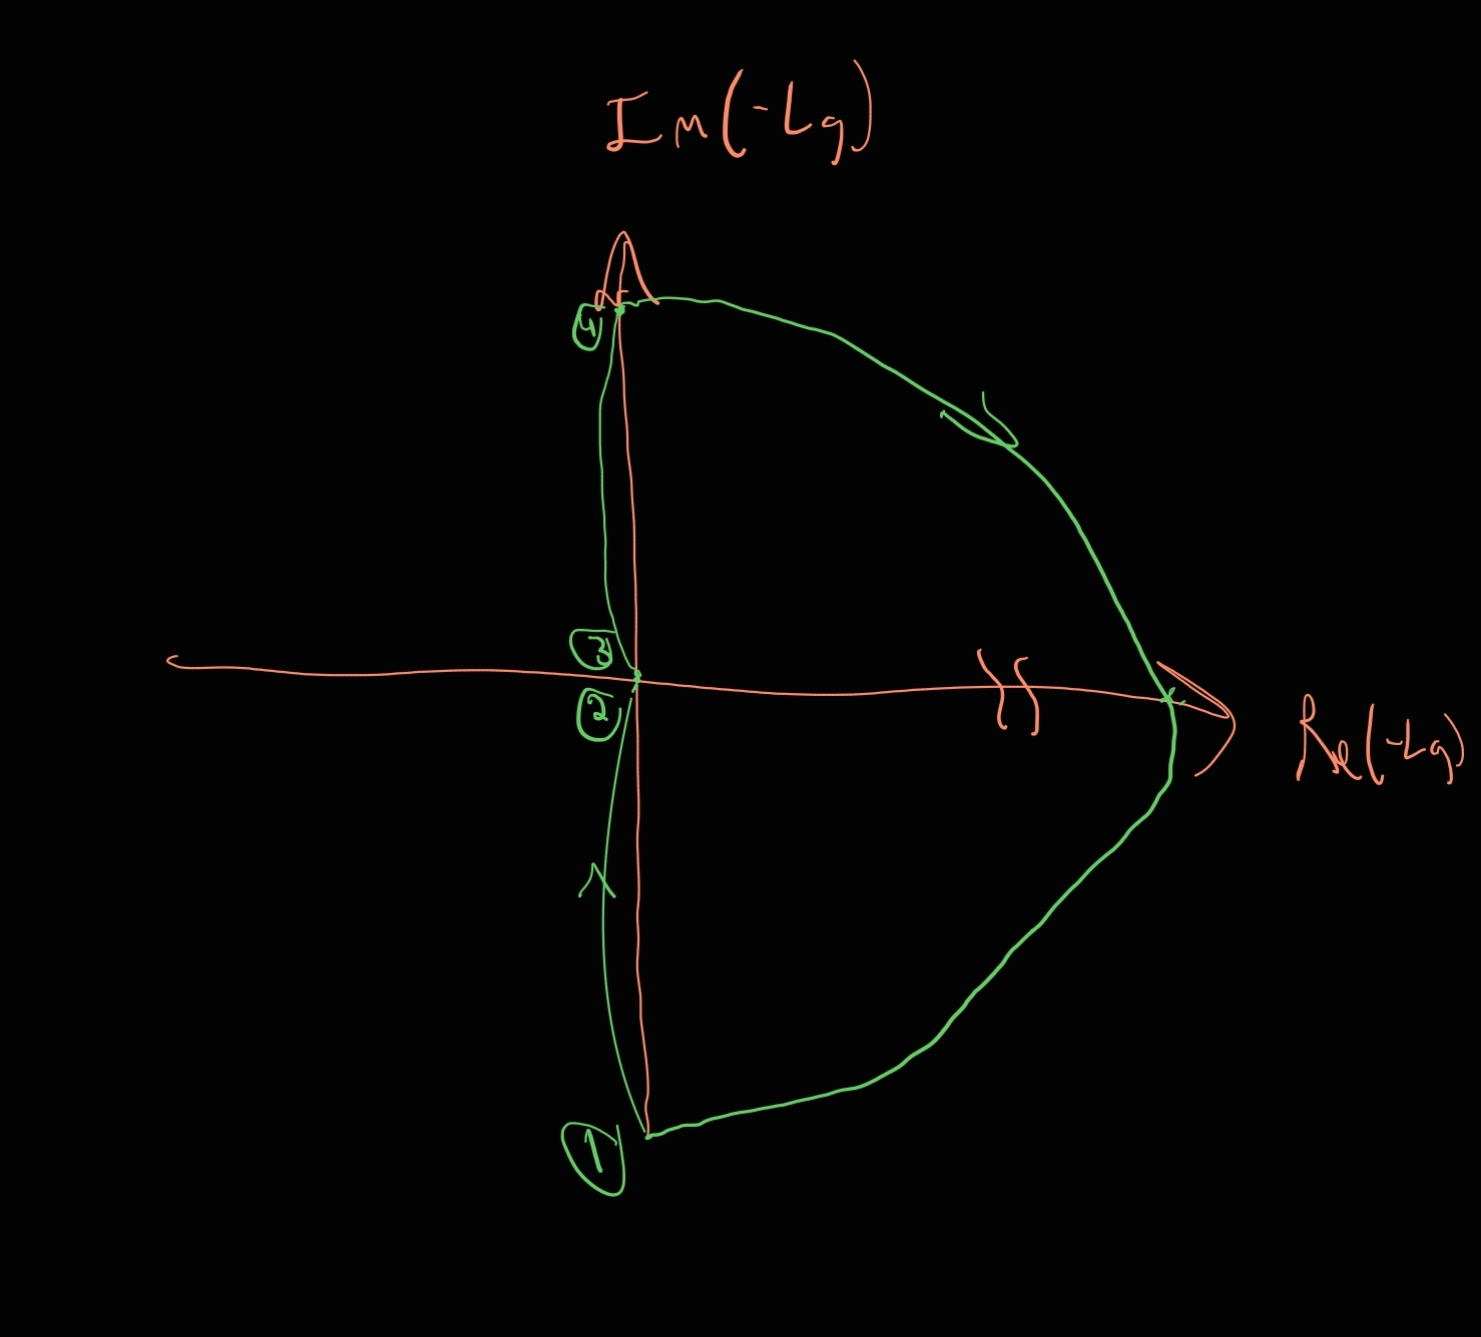
\includegraphics[width=0.8\textwidth]{nyquistDiagram.jpg}
    \label{fig:nyquistDiagram}
    \caption{Nyquist Diagram of Analytic TF}
\end{figure}

As you can see the diagram starts out at point 1 at -90 degrees and negative infinite and then as it goes to point 2 it goes to 0 as the magnitude of the denominator takes over and the 4 poles and 2 zeros sum to -180 degrees as it does so.
Then it goes to point 3 and the magnitude stays big but the phase flips to +90, then the magnitude grows to get to point 4 and as point 4 comes back around to point 1 the phase flips again going from positive 90 to negative 90 and you see that -180 curve around infinite in the diagram.
This means that there are no encirclements at K = 1 and there are no unstable poles in the right half plane so the system is stable there.
As I increase K you can see how that phase margin is shrinking but will never quite touch that stability criterion.

\begin{figure}[H]
    \centering
    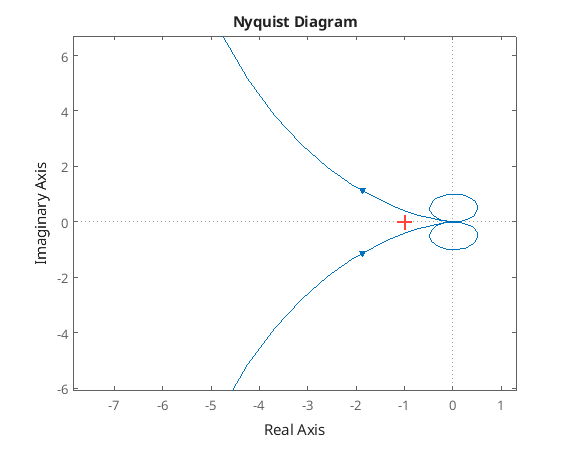
\includegraphics[width=0.8\textwidth]{k10nyquistDiagram.png}
    \label{fig:k10nyquistDiagram}
    \caption{K=10 Nyquist Diagram}
\end{figure}

\begin{figure}[H]
    \centering
    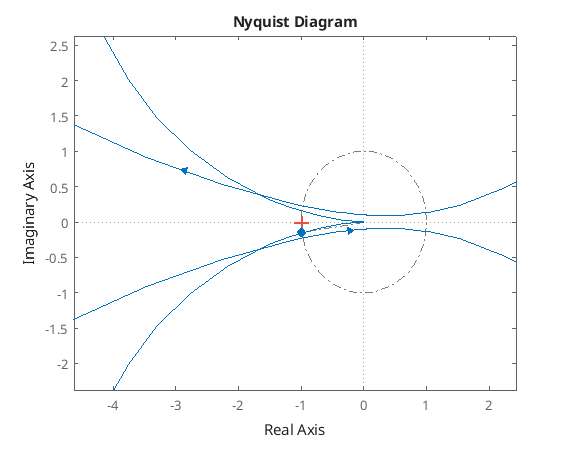
\includegraphics[width=0.8\textwidth]{k100nyquistDiagram.png}
    \label{fig:k100nyquistDiagram}
    \caption{K=100 Nyquist Diagram}
\end{figure}

This corresponds to that gain crossover frequency moving down the Bode plot as the gain increases and the phase margin getting closer and closer to -180 degrees but never quite touching it.

\begin{figure}[H]
    \centering
    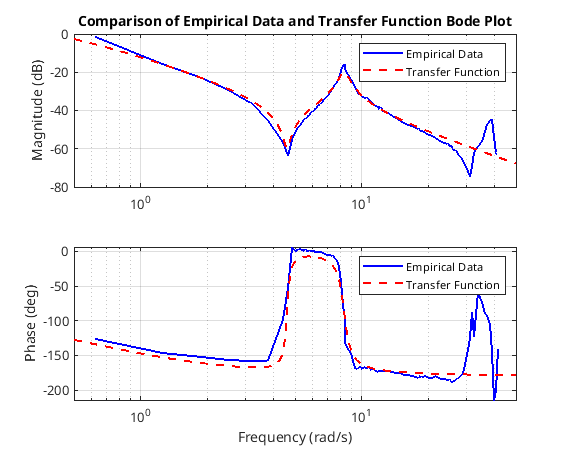
\includegraphics[width=0.8\textwidth]{analyticTFbode.png}
    \label{fig:analyticTFbodePhaseMargin}
\end{figure}

However, the empirical frequency response does cross over -180 degree phase a couple of times and so you would expect that there would be a high gain where you would see a nyquist diagram encirclement and therefore some instability.
Below you can see where I set K to 1000 for the empirical transfer function and how that creates an encirclement.

\begin{figure}[H]
    \centering
    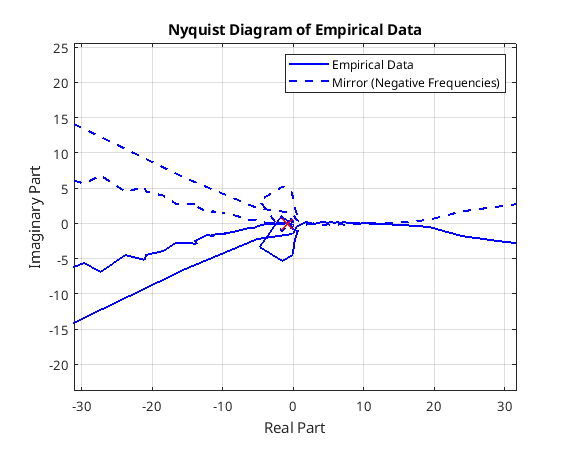
\includegraphics[width=0.8\textwidth]{empiricalK1000zoom.png}
    \label{fig:empiricalK1000zoom}
    \caption{K=1000 Empirical Nyquist Diagram}
\end{figure}

Also, any negative values of K will result in an encirclement of the -1 point and therefore an unstable system.

\begin{figure}[H]
    \centering
    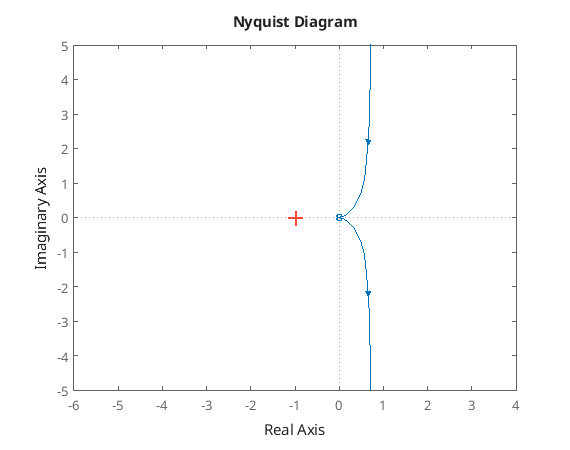
\includegraphics[width=0.8\textwidth]{kNeg1nyquistDiagram.png}
    \label{fig:k-1nyquistDiagram}
    \caption{K=-1 Nyquist Diagram}
\end{figure}

\begin{figure}[H]
    \centering
    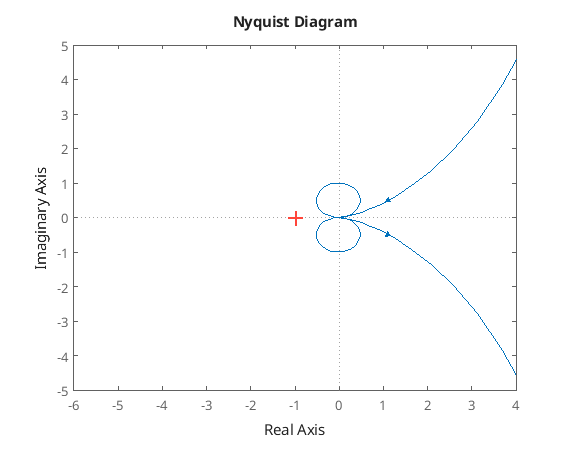
\includegraphics[width=0.8\textwidth]{kNeg10nyquistDiagram.png}
    \label{fig:k-10nyquistDiagram}
    \caption{K=-10 Nyquist Diagram}
\end{figure}

\begin{figure}[H]
    \centering
    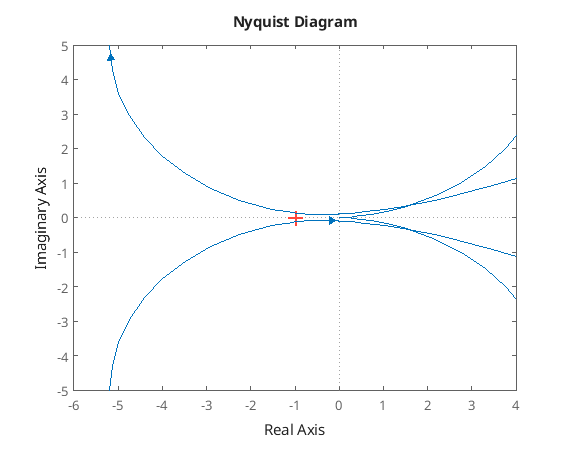
\includegraphics[width=0.8\textwidth]{kNeg100nyquistDiagram.png}
    \label{fig:k-100nyquistDiagram}
    \caption{K=-100 Nyquist Diagram}
\end{figure}

\section{}

\textit{[30 pts] Design a compensator \(C_1(s)\) so that the unity feedback control system with \(C(s) = K C_1(s)\) has at least 40 deg phase margin, 10 dB of gain margin, and a closed loop (-3 dB) bandwidth as close to 1 Hz as possible. Use the analytic plant model in this design. Compute and plot the closed loop tracking frequency response.}

\section{}

\textit{[10 pts] Repeat part 4 using the empirical plant frequency response. Adjust the control design as necessary to try to maintain the stability and performance objectives. Comment on the effects of the unmodeled dynamics at high frequency.}

\section{}

\textit{[20 pts] Simulate the analytic model in a unity feedback control loop in Simulink using the control design from part 4. Plot the responses to a 0.5 rad step input, and to single-sinusoid inputs at 0.5 Hz and 2.0 Hz, each with amplitude 0.5 rad. Also plot the torque input signal, along with its limiting values. Compare these responses with expectations from loop gain analysis for closed loop frequency response, DC tracking accuracy, and stability margins.}

\section{}

\textit{[20 pts – graduate credit only] Suppose the spacecraft had a model where the first resonance occurred before the anti-resonance in frequency. Sketch this Bode plot, and determine if your controller designed in Part 4 would produce a stable system. Comment on the difficulty of achieving the above closed loop stability and tracking bandwidth performance with this “non-colocated” plant.}

\end{document}